%%%%%%%%%%%%%%%%%%%%%%%%%%%%%%%%%%%%%%%%%%%%%%%%%%%%%%%%%%%
% --------------------------------------------------------
% Tau
% LaTeX Template
% Version 2.4.4 (28/02/2025)
%
% Author: 
% Guillermo Jimenez (memo.notess1@gmail.com)
% 
% License:
% Creative Commons CC BY 4.0
% --------------------------------------------------------
%%%%%%%%%%%%%%%%%%%%%%%%%%%%%%%%%%%%%%%%%%%%%%%%%%%%%%%%%%%

\documentclass[9pt,a4paper,twocolumn,twoside]{tau-class/tau}
\usepackage[english]{babel}
\usepackage{lipsum}
\usepackage[utf8]{inputenc}

\usepackage{pgfplots}
\usepackage{siunitx}
\usepgfplotslibrary{fillbetween}
\usetikzlibrary{patterns}  
\pgfplotsset{compat=1.18}


%\usepackage[siunitx]{circuitikz}

%% Spanish babel recomendation
% \usepackage[spanish,es-nodecimaldot,es-noindentfirst]{babel} 

%% Draft watermark
% \usepackage{draftwatermark}

%----------------------------------------------------------
% TITLE
%----------------------------------------------------------

\journalname{Torino, 5 giugno 2025}
\title{Esperienza di laboratorio: Diodi}

%----------------------------------------------------------
% AUTHORS, AFFILIATIONS AND PROFESSOR
%----------------------------------------------------------

\author[b,c,3]{Mattia Benna, Federico Cesari, Matteo Herz}

%----------------------------------------------------------

%\affil[a]{Affiliation of author one}
%\affil[b]{Affiliation of author two}
%\affil[c]{Affiliation of author three}

\professor{Università di Torino - Corso di Laurea in Fisica}

%----------------------------------------------------------
% FOOTER INFORMATION
%----------------------------------------------------------

\institution{Unito fisica}
\theday{5 giugno, 2025}
\course{Esperimentazioni 2}


%----------------------------------------------------------
% ABSTRACT AND KEYWORDS
%----------------------------------------------------------

\begin{abstract}
%In questa esperienza di laboratorio abbiamo studiato la caratteristica corrente-tensione di due diodi, uno al silicio e uno LED. I risultati ottenuti sono stati confrontati con le previsioni teoriche, permettendo di verificare la coerenza dell'andamento misurato sperimentalmente con le due equazioni teoriche illustrate al punto 2.
%Infine abbiamo verificato qualitativamente l'utilizzo di un diodo accoppiato con un filtro RC per il raddrizzamento di una semionda.
In questa esperienza di laboratorio è stata studiata la caratteristica corrente-tensione di due diodi: uno al silicio ed uno LED. I dati ottenuti sono stati confrontati attraverso vari fit con le previsioni teoriche, verificando la coerenza dell'andamento misurato sperimentalmente con le equazioni teoriche illustrate al punto [\ref{sec:2}].
Infine, è stato verificato qualitativamente l'utilizzo del diodo accoppiato ad un filtro RC per il raddrizzamento di una semionda.


\end{abstract}

%----------------------------------------------------------

%\keywords{filtro passa-banda, circuito RLC, guadagno}

%----------------------------------------------------------

\begin{document}
		
    \maketitle 
    \thispagestyle{firststyle} 
    \tauabstract
    % \tableofcontents
    % \linenumbers 
    
%----------------------------------------------------------
%\vspace{-0.8cm}
\section{Introduzione}
I diodi sono componenti elettronici fondamentali che consentono il passaggio della corrente in una sola direzione, comportandosi come interruttori unidirezionali. Questo comportamento deriva dalla loro giunzione PN, la cui risposta elettrica varia in base alla polarizzazione (diretta o inversa), generando una caratteristica tensione-corrente non lineare.
I diodi trovano ampio impiego in elettronica: dal raddrizzamento di segnali alternati, alla stabilizzazione di tensione (diodi Zener), alla protezione dei circuiti (diodi di blocco o soppressione), fino all'emissione luminosa nei diodi LED (\textit{Light Emitting Diode}).

\section{Nozioni teoriche}\label{sec:2}
I diodi sono dispositivi elettronici formati da una giunzione tra due semiconduttori drogati, uno di tipo \textbf{P} e uno di tipo \textbf{N}. Questa struttura permette il passaggio della corrente solo in una direzione. A differenza delle resistenze, la direzione in cui si collega un diodo è fondamentale per il suo funzionamento.

Quando il diodo non è collegato a una sorgente esterna, nella giunzione PN si crea uno stato di equilibrio con una tensione interna fissa, chiamata \textit{tensione di built-in}.

Inserendo il diodo in un circuito, si possono distinguere due casi:

\begin{itemize}
    \item \textbf{Polarizzazione diretta:} il lato P è collegato al polo positivo e il lato N al negativo; la barriera di potenziale si riduce e il diodo permette il passaggio della corrente.
    
    \item \textbf{Polarizzazione inversa:} il collegamento è opposto; la barriera di potenziale aumenta e blocca il passaggio dei portatori di carica maggioritari. In questo caso può comunque fluire una debole corrente, detta \textit{corrente di saturazione inversa} (\( I_s \)), dovuta ai portatori minoritari.
\end{itemize}


La relazione che descrive la corrente in funzione della tensione a cui è soggetto il diodo è non lineare ed è descritta dall'equazione di Shockley:

\begin{equation}
      I_d=I_s \left(e^{\frac{V_d}{\eta V_T}}-1\right) \hspace{15pt} V_T=\frac{kT}{e}
      \label{eq:Id}
\end{equation}

dove $I_s$ è la corrente di saturazione inversa, $\eta$ è il fattore di idealità, $k$ è la costante di Boltzmann, $e$ è la carica dell'elettrone e $T$ è la temperatura. Ad una temperatura di 300K il valore di $V_T$ vale circa 26 mV (valore che verrà utilizzato in fase di analisi dati).\\
Nel caso dei diodi LED, è presente una particolarità aggiuntiva: questi dispositivi mostrano una \textit{componente resistiva} non trascurabile, indicata con \( R_d \). Tale resistenza è legata sia alla struttura fisica del diodo sia agli effetti termici che si manifestano durante il funzionamento.

Per questo motivo, la caduta di tensione ai capi del diodo LED non può essere descritta completamente dalla sola equazione di Shockley, che considera un diodo ideale.

E' però possibile ricavare l'andamento della tensione in funzione della corrente, invertendo la legge di Shockley e aggiungendo il termine di caduta di potenziale:

\begin{equation}
    V_d=\eta V_T \ln\left(\frac{I_d}{I_s}+1\right)+R_dI_d
    \label{eq:Vd}
\end{equation}

\section{Apparato e procedura sperimentale}

\subsection{Apparato sperimentale}
In laboratorio è stata utilizzata la seguente attrezzatura:
\begin{itemize}
    \item 2 Diodi: uno LED e uno al silicio
    \item Resistenze comprese fra 1 e 5 K$\Omega$
    \item Tester Amprobe 37XR-A
    \item Generatore di funzioni Siglent SDG1062X Plus
    \item Oscilloscopio Tektronix 2002
    \item Condensatore variabile
    \item Basetta per circuiti elettrici 
\end{itemize} 

\noindent Con tale strumentazione sono stati riprodotti su basetta i seguenti circuiti: 
\begin{figure}[H]
\centering
   \begin{circuitikz}
    \draw (0,0) to[V, l=$V_{DC}$] (0,3) -- (2,3)
    to[R, l=$R$] (4,3) -- (5,3)
    to[diode, l=D] (5,0) -- (0,0);
    \draw (5,3) -- (7,3)
    to[voltmeter, l=$V_{out}$] (7,0) -- (5,0);
    \end{circuitikz}
\caption{Circuito per caratteristica I-V diodi}
\label{fig:1}
\end{figure}
\begin{figure}[H]
\centering
   \begin{circuitikz}
     \draw (0,0) to[sV, l=$V_{AC}$] (0,3) -- (2,3)
    to[diode, l=D] (4,3) -- (5,3)
    to[C, l=$C$] (5,0) -- (0,0);
    \draw (5,3) -- (7,3)
    to[R, l=$R$] (7,0) -- (5,0);
    \end{circuitikz}
\caption{Circuito per raddrizzamento della semionda}
\label{fig:2}
\end{figure}

\subsection{Procedura sperimentale}

L’attività sperimentale si è articolata in due fasi distinte:
\begin{enumerate}
    \item la caratterizzazione della curva I-V di due differenti diodi (al silicio e LED);
    \item lo studio qualitativo del raddrizzamento di una semionda tramite l’utilizzo di un circuito con diodo e filtro $RC$.
\end{enumerate}

Per la prima parte, è stato utilizzato un circuito in polarizzazione diretta come illustrato in Fig.[\ref{fig:1}], alimentato da un generatore di tensione continua. Una resistenza da $(2.72 \pm 0.03)\, k\Omega$ è stata inserita in serie al diodo per limitarne la corrente, e le misure sono state effettuate in coppia (tensione ai capi del diodo $V_d$ e corrente $I_d$) variando progressivamente il valore di $V_{in}$ da 0 V a 10/20 V.

Il milliamperometro e il voltmetro sono stati scelti con attenzione, in particolare assicurandosi che la resistenza interna del voltmetro fosse sufficientemente elevata per garantire che $I \simeq I_d$.\\Il procedimento di raccolta dati per il LED è stato del tutto analogo a quello usato per il diodo al silicio.\\ 

Nella seconda fase dell’esperimento, per studiare il comportamento del diodo come raddrizzatore, è stato costruito un circuito alimentato da un generatore di tensione alternata, come mostrato in Fig[\ref{fig:2}]. In questo caso il segnale in ingresso $V_{in}$ e quello in uscita $V_{out}$ sono stati visualizzati tramite oscilloscopio.

Per osservare l'effetto di raddrizzamento della semionda è stato inserito un filtro RC in serie al diodo. Variando la costante di tempo $\tau = RC$ (grazie all'uso di resistori e condensatori variabili), è stato possibile verificare come l'onda raddrizzata tendesse a trasformarsi in un segnale continuo al crescere di $\tau$, confermando il ruolo importante del diodo nella conversione AC–DC.
\section{Analisi dati e discussione}
\subsection{Diodo al silicio}
Dai dati ottenuti in laboratorio è stato possibile ricavare la caratteristica I-V per il diodo al silicio. Di seguito il grafico ottenuto dal fit ed i relativi parametri. 

\begin{figure}[H]
  \centering
  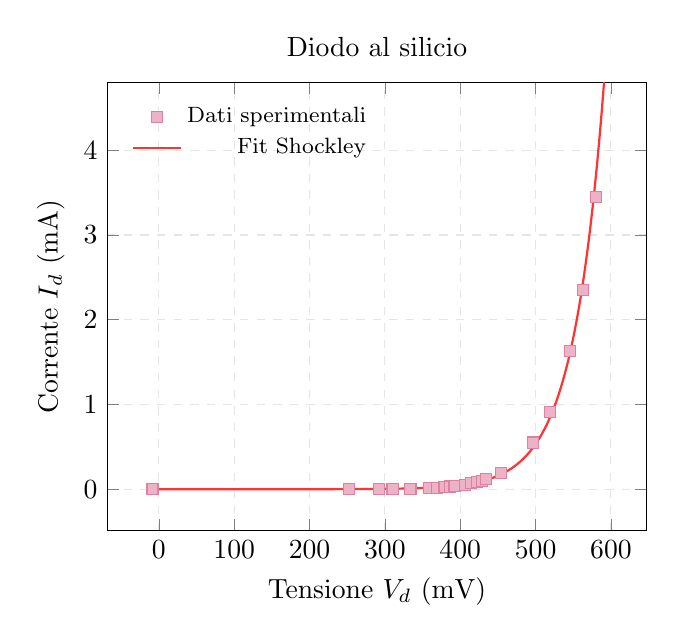
\begin{tikzpicture}
		\begin{axis}[
			title={Diodo al silicio},
			xlabel={Tensione \(V_d\) (mV)},
			ylabel={Corrente \(I_d\) (mA)},
                ymax = 4.8,
			grid=both,
			grid style={dashed, gray!20},
			legend pos=north west,
			error bars/x dir=both,
			error bars/y dir=both,
			error bars/x explicit,
			error bars/y explicit,
                legend style={
                    draw=none,
                    fill=none,
                    text opacity=1,
                    font=\footnotesize,
                    cells={anchor=east}
                }
			]
			
			% Dati con errori
			\addplot+ [
			only marks,
			mark=square*,
			mark options={solid, fill=purple!30, draw=purple!50, scale=1},
			] table [x error=x_v_err, y error=y_i_err] {
				x       y       x_v_err   y_i_err
				-8.4	0	0.458	0.01
                    252.4	0	1.762	0.005
                    292.4	0.002	1.962	0.00501
                    310.2	0.003	2.051	0.005015
                    333.9	0.007	2.1695	0.005035
                    358.8	0.014	2.294	0.00507
                    369.4	0.017	2.347	0.005085
                    379.2	0.026	2.396	0.00513
                    386	0.031	2.43	0.005155
                    392.4	0.038	2.462	0.00519
                    405.9	0.053	2.5295	0.005265
                    414.5	0.071	2.5725	0.005355
                    422.4	0.083	2.612	0.005415
                    428.6	0.098	2.643	0.00549
                    433.8	0.117	2.669	0.005585
                    454.4	0.196	2.772	0.00598
                    496.5	0.551	2.9825	0.007755
                    519.2	0.909	3.096	0.009545
                    545.4	1.635	3.227	0.013175
                    563.2	2.354	3.316	0.01677
                    580.5	3.447	3.4025	0.022235
			
			};
                \addplot[
			red!80, 
			thick, 
			domain=0:600, 
			samples=200
			] {
				2.98*pow(10,-6)*(exp(x/(1.59*26)) - 1)
			};
			\addlegendentry{Dati sperimentali}
                \addlegendentry{Fit Shockley}
		\end{axis}
	\end{tikzpicture}
  \caption{Caratteristica \( I_d(V_d) \)}
  \label{fig:ledfit}
\end{figure}

\begin{table}[H]
            \centering
            \begin{tabular}{cc}
                \toprule
                $\chi^2$/ndf & \(10.13/18\) \\
                $I_s$ & $(2.98 \pm 0.56)\cdot 10^{-6}\text{ mA}$ \\
                $\eta$ & $\;\;\;\;1.59 \pm 0.03 \text{ }$\\
                \bottomrule
            \end{tabular}
            \caption{Parametri fit}
\end{table}

Dal grafico è visibile l'accordo tra l'andamento dei dati ricavati in laboratorio e l'equazione di Shockley. Il valore ottenuto per il $\chi^2$ conferma quanto si osserva dal grafico. Inoltre i valori dei parametri ottenuti dal fit sono coerenti con quanto atteso: una corrente di saturazione $I_s$ nell'ordine dei milliampere ed un valore di $\eta$ non distante da 2 (valore teorico). 

\subsection{Diodo LED}
Tenendo conto della componente resistiva non trascurabile del diodo LED, dai dati ottenuti in laboratorio si è ricavato l'andamento $V_d(I_d)$, come descritto dall'equazione [\ref{eq:Vd}].  Di seguito il grafico ottenuto dal fit ed i relativi parametri.

\begin{figure}[H]
  \centering
  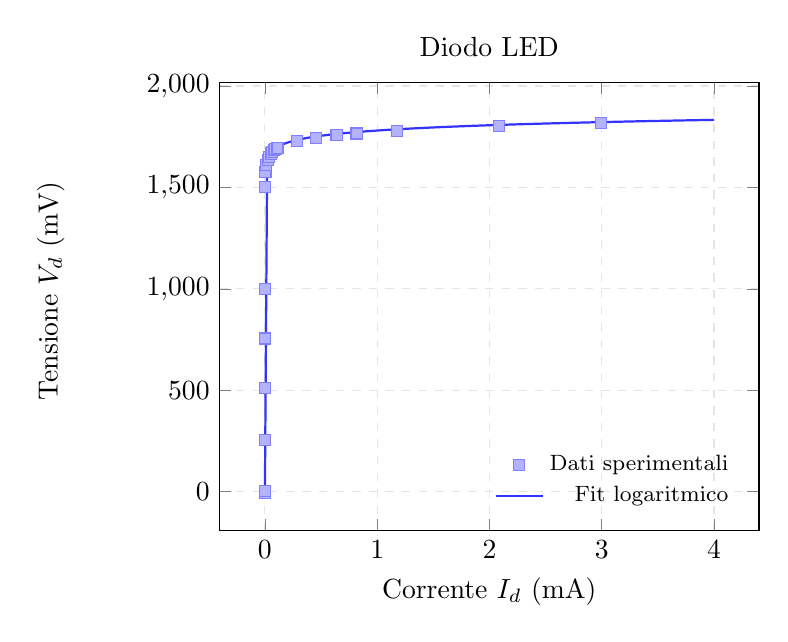
\begin{tikzpicture}
		\begin{axis}[
			title={Diodo LED},
			ylabel={Tensione \(V_d\) (mV)},
                ylabel style={shift={(0.2cm,0.8cm)}},
			xlabel={Corrente \(I_d\) (mA)},
			grid=both,
			grid style={dashed, gray!20},
			legend pos=south east,
			error bars/x dir=both,
			error bars/y dir=both,
			error bars/x explicit,
			error bars/y explicit,
                legend style={
                    draw=none,
                    fill=none,
                    text opacity=1,
                    font=\footnotesize,
                    cells={anchor=east}
                }
			]
			
			% Dati con errori
			\addplot+ [
			only marks,
			mark=square*,
			mark options={solid, fill=blue!30, draw=blue!50, scale=1},
			] table [x error=x_v_err, y error=y_i_err] {
			x       y        x_v_err  y_i_err  
			0	-8.6	0.005	0.457
                0	255.3	0.005	1.7765
                0	509.8	0.005	3.049
                0	755.1	0.005	4.2755
                0	1001	0.005	5.505
                0	1.19	0.005	0.50595
                0	1.353	0.005	0.506765
                0.001	1501	0.005005	8.005
                0.005	1577	0.005025	8.385
                0.013	1611	0.005065	8.555
                0.024	1637	0.00512	8.685
                0.036	1652	0.00518	8.76
                0.052	1667	0.00526	8.835
                0.064	1675	0.00532	8.875
                0.079	1683	0.005395	8.915
                0.094	1690	0.00547	8.95
                0.112	1695	0.00556	8.975
                0.285	1729	0.006425	9.145
                0.458	1745	0.00729	9.225
                0.638	1757	0.00819	9.285
                0.816	1766	0.00908	9.33
                1.177	1780	0.010885	9.4
                2.086	1803	0.01543	9.515
                2.994	1818	0.01997	9.59
			};
                \addlegendentry{Dati sperimentali}
                \addplot[
			blue!80, 
			thick, 
			domain=0:4, 
			samples=200
			] {
				1.42*26*ln(x/(1.15*pow(10,-21)) + 1 ) + 0.49*x
			};
                \addlegendentry{Fit logaritmico}
		
		\end{axis}
	\end{tikzpicture}
  \caption{Caratteristica \( V_d(I_d) \)}
  \label{fig:ledfit}
\end{figure}

\begin{table}[H]
            \centering
            \begin{tabular}{cc}
                \toprule
                $\chi^2$/ndf & \(0.33/21\) \\
                $I_s$ & $(1.15 \pm 1.73)\cdot 10^{-21}\text{ mA}$ \\
                $\eta$ & $\;\;\;\;1.42 \pm 0.04 $\\
                $R_d$  & $0.49 \pm 3.48 \,\Omega$\\
                \bottomrule   
            \end{tabular}
            \caption{Parametri fit}
\end{table}

L'andamento teorico descritto dall'equazione [\ref{eq:Vd}] è in accordo con quello dei dati ottenuti in laboratorio per il diodo LED. L'accordo è sottolineato anche in questo caso da un valore del $\chi^2$ accettabile.
I valori ottenuti per gli altri parametri di fit risultano coerenti con quanto atteso: un fattore di idealità $\eta$ compreso tra 1 e 2 ed una corrente di saturazione molto bassa.

Il valore della resistenza del diodo ($R_d$) risulta poco superiore allo zero e al massimo, considerando l'incertezza ottenuta, del valore di qualche Ohm\footnote{Tenendo conto dell'incertezza associata alla resistenza (dato puramente matematico estratto dal fit) è da considerare solo il caso fisicamente sensato in cui $R_d \geq 0$}.
Per visualizzare l'effettiva trascurabilità o meno di tale componente resistiva, possiamo osservare i parametri del fit ottenuti per il diodo LED utilizzando direttamente l'equazione [\ref{eq:Id}], non tenente conto di $R_d$:

\begin{figure}[H]
  \centering
  \begin{tikzpicture}
		\begin{axis}[
			title={Diodo LED},
			xlabel={Tensione \(V_d\) (mV)},
			ylabel={Corrente \(I_d\) (mA)},
			grid=both,
                ymax = 4.5,
			grid style={dashed, gray!20},
			legend pos=north west,
			error bars/x dir=both,
			error bars/y dir=both,
			error bars/x explicit,
			error bars/y explicit,
                legend style={
                    draw=none,
                    fill=none,
                    text opacity=1,
                    font=\footnotesize,
                    cells={anchor=east}
                }
			]
			
			% Dati con errori
			\addplot+ [
			only marks,
			mark=square*,
			mark options={solid, fill=blue!30, draw=blue!50, scale=1},
			] table [x error=x_v_err, y error=y_i_err] {
				x       y       x_v_err   y_i_err
				-8.6	0	0.457	0.005
                    255.3	0	1.7765	0.005
                    509.8	0	3.049	0.005
                    755.1	0	4.2755	0.005
                    1001	0	5.505	0.005
                    1.19	0	0.50595	0.005
                    1.353	0	0.506765	0.005
                    1501	0.001	8.005	0.005005
                    1577	0.005	8.385	0.005025
                    1611	0.013	8.555	0.005065
                    1637	0.024	8.685	0.00512
                    1652	0.036	8.76	0.00518
                    1667	0.052	8.835	0.00526
                    1675	0.064	8.875	0.00532
                    1683	0.079	8.915	0.005395
                    1690	0.094	8.95	0.00547
                    1695	0.112	8.975	0.00556
                    1729	0.285	9.145	0.006425
                    1745	0.458	9.225	0.00729
                    1757	0.638	9.285	0.00819
                    1766	0.816	9.33	0.00908
                    1780	1.177	9.4	0.010885
                    1803	2.086	9.515	0.01543
                    1818	2.994	9.59	0.01997
			
			};
                \addplot[
			blue!80, 
			thick, 
			domain=0:2000, 
			samples=200
			] {
				1.22*pow(10,-21)*(exp(x/(1.412*26)) - 1)
			};
			\addlegendentry{Dati sperimentali}
                \addlegendentry{Fit Shockley}
		\end{axis}
	\end{tikzpicture}
  \caption{Caratteristica \( I_d(V_d) \) per il diodo LED}
  \label{fig:ledfit}
\end{figure}

\begin{table}[H]
            \centering
            \begin{tabular}{cc}
                \toprule
                $\chi^2$/ndf & \(0.34/21\) \\
                $I_s$ & $(1.22 \pm 2.75)\cdot 10^{-21}\text{ mA}$ \\
                $\eta$ & $\;\;\;\;1.412 \pm 0.001 $\\
                $R_d$  & $0.48 \pm 3.48 \,\Omega$\\
                \bottomrule   
            \end{tabular}
            \caption{Parametri fit}
\end{table}

Dai risultati ottenuti si evince come anche l'equazione di Shockley [\ref{eq:Id}] descrive sufficiente bene l'andamento dei dati sperimentali. Tale fit ha infatti restituito parametri compatibili con quanto osservato tenendo invece conto dell'equazione [\ref{eq:Vd}]. 

Si suppone che l'effetto resistivo del diodo sarebbe stato più evidente a voltaggi di lavoro più alti di quelli utilizzati durante l'esperienza di laboratorio. 

% \subsection{Raddrizzamento di una semionda}
 
\section{Conclusioni}
I grafici ottenuti per le caratteristiche I–V dei due diodi mostrano un buon accordo con l'andamento teorico descritto dall'equazione di Shockley [\ref{eq:Id}] e dall'equazione [\ref{eq:Vd}], confermando la validità del modello anche nel caso del LED, nonostante la presenza di una diversa soglia di conduzione e di una componente resistiva maggiore.\\
I parametri ottenuti tramite regressione risultano coerenti con i valori attesi dalla teoria, indicando una buona qualità delle misure svolte in laboratorio.\\
È stato inoltre riprodotto ed osservato con successo il fenomeno del raddrizzamento di una semionda combinando il diodo con un filtro RC. 

\end{document}